\documentclass{../ape}

\usepackage{../../linma2345}

\begin{document}

\session{11}{Coalitions}

%\textbf{Session 11:  Coalitions}

%\section*{Exercices}


%\newpage

\section{} Alice, Bob and Carol wish to connect to the Internet. The cost of such a connection depends on the total length of cables that it requires. Of course, the players also need to be connected to the provider $\Omega$. The costs of the possible connections are given by the following graph.
\begin{figure}[!ht]
	\begin{center}
		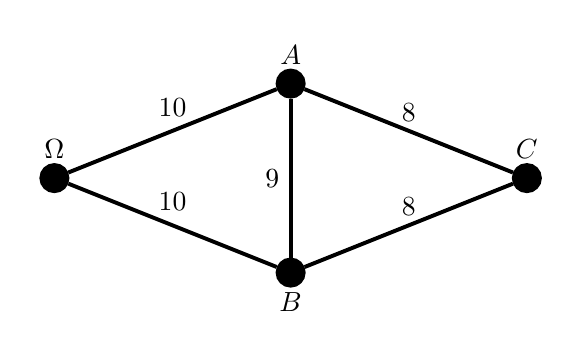
\begin{tikzpicture}[scale=2,looseness=.8,auto]
			\begin{scope}[every node/.style={font=\small\itshape},line width=0.5mm]
				\tikzstyle{every node}=[draw,fill=black,shape=circle,line width=0.5mm,minimum size=1.5mm,label distance=1mm];
				\path (0  , 0  ) node (v0) {} node [above,draw=none,fill=none] {$\Omega$};
				\path (1.5,  .6) node (vA) {} node [above,draw=none,fill=none] {$A$};
				\path (1.5, -.6) node (vB) {} node [below,draw=none,fill=none] {$B$};
				\path (3  , 0  ) node (vC) {} node [above,draw=none,fill=none] {$C$};
				\draw (v0) -- (vA) node [midway,above,draw=none,fill=none,yshift=-1mm] {$10$};
				\draw (v0) -- (vB) node [midway,above,draw=none,fill=none,yshift=-1mm] {$10$};
				\draw (vA) -- (vB) node [midway,left,draw=none,fill=none,xshift=1mm] {$9$};
				\draw (vA) -- (vC) node [midway,above,draw=none,fill=none,yshift=-1mm] {$8$};
				\draw (vB) -- (vC) node [midway,above,draw=none,fill=none,yshift=-1mm] {$8$};
			\end{scope}
		\end{tikzpicture}
	\end{center}
\end{figure}

Therefore, connecting all the players has a total cost of 26, an amount that they then need to share. Furthermore, for each player, being connected to the Internet represents a profit of 20.
\begin{enumerate}
	\item[a.] If the players can agree on a division of connection fees, what solution do you propose?
%	what is the \emph{core} in which they will choose their individual costs?
	\item[b.] Suppose you were the provider, and that you wanted to impose costs that are as honest as possible. How would you divide the costs?
\end{enumerate}

\begin{solution}
\begin{enumerate} [label=\alph*.]
	%%%%%% a
	\item First, let us give a little bit of intuition.
	Let us imagine three cases. As often, we use $x_{A}$, $x_{B}$ and $x_{C}$ to denote the payoff of Alice, Bob and Carol, respectively.
	
	\paragraph{Case 1. The three players play together.}
	In this case, the selected edges will be $\parent{\Omega, A}$, $\parent{A, C}$ and $\parent{B, C}$. The total cost is 26. Each player will have a profit of 20, hence the total profit is 60. This means that the final, total payoff is $60 - 26 = 34$. This payoff is then shared amongst the three players, hence we have
	\begin{equation*}
	    x_{A} = x_{B} = x_{C} = \dfrac{34}{3} = 11.333.
	\end{equation*}
	
	\paragraph{Case 2. The two players $A$ and $B$ play together.}
	In this case, the selected edges will be $\parent{\Omega, A}$ and $\parent{A, B}$. The total cost is 19. Each player will have a profit of 20, hence the total profit is 40. This means that the final, total payoff is $40 - 19 = 21$. This payoff is then shared amongst the two players, hence we have
	\begin{equation*}
	    x_{A} = x_{B} = \dfrac{21}{2} = 10.5.
	\end{equation*}
	
	
	\paragraph{Case 3. Player $A$ plays alone.}
	In this case, the selected edge will be $\parent{\Omega, A}$. The total cost is 10. Each player will have a profit of 20, hence the total profit is 20. This means that the final, total payoff is $20 - 10 = 10$. This payoff does not have to be shared, because player $A$ is alone, hence we have
	\begin{equation*}
	    x_{A} = 10.
	\end{equation*}
	
	We see that Case 1 is preferable to Case 2, which is preferable to Case 3, for player $A$. A similar discussion can be made for players $B$ and $C$. 
	
	
	\vspace{5mm}
	
	In order to discuss things more formally, let us construct $v$, the characteristic function. How many subsets do we have? We have $\phi$, $\bracket{A}$, $\bracket{B}$, $\bracket{C}$, $\bracket{A, B}$, $\bracket{A, C}$, $\bracket{B, C}$ and $\bracket{A, B, C}$, hence we have 8 subsets.
	
	We can easily compute that
	\begin{align*}
	    & v \parent{\phi} = 0 - 0 = 0 \\ \\
	    & v \parent{\bracket{A}} = 20 - 10 = 10 \\
	    & v \parent{\bracket{B}} = 10 \text{ (by symmetry) } \\
	    & v \parent{\bracket{C}} = 20 - (10 + 8) = 2 \\ \\
	    & v \parent{\bracket{A, B}} = 2 \cdot 20 - (10 + 9) = 21 \\
	    & v \parent{\bracket{B, C}} = 2 \cdot 20 - (10 + 8) = 22 \\
	    & v \parent{\bracket{A, C}} = 22 \text{ (by symmetry) } \\ \\
	    & v \parent{\bracket{A, B, C}} = 60 - (10 + 8 + 8) = 34
	\end{align*}
	
	We can write the following constraints
	\begin{align*}
	    & 10 \leq x_{A} \\
	    & 10 \leq x_{B} \\
	    & 2 \leq x_{C} \\ \\
	    & 21 \leq x_{A} + x_{B} \\
	    & 22 \leq x_{B} + x_{C} \\
	    & 22 \leq x_{A} + x_{C} \\ \\
	    & 34 = x_{A} + x_{B} + x_{C} \\
	\end{align*}
	
	By manipulating these constraints, we can add a couple of constraints. For example, we have $21 \leq x_{A} + x_{B}$. By adding $x_{C}$ on both sides, and using the fact that $34 = x_{A} + x_{B} + x_{C}$, we can find the extra constraint $x_{C} \leq 13$. Using a similar argument, we can find the following constraints
	\begin{align*}
	    & x_{A} \leq 12 \\
	    & x_{B} \leq 12 \\
	    & x_{C} \leq 13 \\
	\end{align*}
	
	Furthermore, we can take $x_{A} \leq 12$ and add $x_{C}$ on both sides, again, to obtain $x_{A} + x_{C} \leq 12 + x_{C}$. Using the fact that $22 \leq x_{A} + x_{C}$, we obtain $22 \leq 12 + x_{C}$, hence $10 \leq x_{C}$, which is more precise than $2 \leq x_{C}$.
	
	Putting everything together, we can define the core of our problem
	\begin{align}
	    & 10 \leq x_{A} \leq 12 \label{eq:coreA} \\
	    & 10 \leq x_{B} \leq 12 \label{eq:coreB} \\
	    & 10 \leq x_{C} \leq 13 \label{eq:coreC} \\
	    & 34 = x_{A} + x_{B} + x_{C} \label{eq:coreSum}
	\end{align}
	
	This looks paradoxical, because player $C$ seems to be advantaged, since the upper bound on $x_{C}$ is higher than the upper bound on $x_{A}$ or $x_{B}$. We wouldn't expect player $C$ to have a higher payoff, since he is the farthest from the source $\Omega$.
	
	Now we ask ourselves: is there an allocation such that all these constraints are true? If yes, then we can propose a solution to the question. If no, then the feasible set will be empty. We can easily see that $\parent{x_{A}, x_{B}, x_{C}} = \parent{12, 12, 10}$ is a valid allocation, as well as $\parent{\dfrac{34}{3}, \dfrac{34}{3}, \dfrac{34}{3}}$. 
	
	
	%%%%% b
	\item In order to find the most honest division of the costs, let us compute the Shapley value. For this, we have two methods. The first method is very intuitive and is based on a large table. The second method is very theoretical, and is based on a complicated formula.
	\paragraph{Method 1. Compute the Shapley value with a table.}
	
	We will construct a table with triplets, say $ACB$. Such a triplet indicates the order in which the players arrive in the game. Hence, the triplet $ACB$ means that first, player $A$ was alone, and he did his best to connect to the Internet. Then, player $C$ arrived in the game: he saw which choices player $A$ had made, and knowing that, he also did his best to connect to the Internet. Finally, player $B$ arrived in the game: he saw which choices players $A$ and $C$ had made, and knowing that, he also did his best to connect to the Internet. In this configuration, we would have
	\begin{itemize}
	    \item Player $A$ enters the game alone. He wins 20, he pays 10, and his payoff is $20 - 10 = 10$.
	    \item Player $C$ enters the game after that. The payoff is $v \parent{\bracket{A, C}} = 22$, and since player $A$ only takes 10, the payoff of player $C$ is $22 - 10 = 12$.
	    \item Player $B$ enters the game after that. The payoff is $v \parent{\bracket{A, B, C}} = 34$, and since players $A$ and $C$ only take 10 and 12 respectively, the payoff of player $B$ is $34 - 10 - 12 = 12$.
	\end{itemize}
	
	Hence, if the triplet is $ACB$, we find $x_{A} = 10$, $x_{B} = 12$ and $x_{C} = 12$.
	
	If we do this for all the triplets, we find the results given on Table \ref{tab:1001payoffs}. We know that there are $3! = 6$ triplets.
	
	
\begin{tabular}[h!]{r|ccccc}
    & $x_{A}$ && $x_{B}$ && $x_{C}$ \\ \hline
$ABC$ & 10 && 11 && 13 \\
$ACB$ & 10 && 12 && 12 \\
$BAC$ & 11 && 10 && 13 \\
$BCA$ & 12 && 10 && 12 \\
$CAB$ & 20 && 12 && 2  \\
$CBA$ & 12 && 20 && 2 \\
\end{tabular}
\captionof{table}{Payoff of each player, in function of the triplet}
\label{tab:1001payoffs}


The final step of Method 1 is to compute the mean of these payoffs. We use $\phi_{A}$, $\phi_{B}$ and $\phi_{C}$ to denote the expected payoff of player $A$, $B$ and $C$, respectively. We find
\begin{align*}
    & \phi_{A} = \dfrac{1}{6} \parent{10 + 10 + 11 + 12 + 20 + 12} = \dfrac{75}{6} = 12.5 \\
    & \phi_{B} = \dfrac{1}{6} \parent{11 + 12 + 10 + 10 + 12 + 20} = \dfrac{75}{6} = 12.5 \\
    & \phi_{C} = \dfrac{1}{6} \parent{13 + 12 + 13 + 12 + 2 + 2} = \dfrac{54}{6} = 9.
\end{align*}
	   
	
	\paragraph{Method 2. Compute the Shapley value with the formula.}
	
	In the reminders, we are told that the Shapley values can be explicitly computed by
	\begin{align*}
		\phi_{i} \parent{v} = \sum_{S \subseteq N -i}{\dfrac{\abs{S}! \parent{\abs{N} - \abs{S} - 1}!}{\abs{N}!} \parent{v \parent{S \cup \bracket{i}} - v \parent{S}}}.
	\end{align*}
	
	We know that $N = \bracket{A, B, C}$. Hence, we can compute
	\begin{align*}
	    \phi_{A} \parent{v}
	    &= \sum_{S \subseteq \bracket{B, C}}{\dfrac{\abs{S}! \parent{3 - \abs{S} - 1}!}{6} \parent{v \parent{S \cup \bracket{A}} - v \parent{S}}}.
	\end{align*}
	
	The sum will consist of four terms
	\begin{enumerate}
	    \item[1.] $S = \phi$
	    \item[2.] $S = \bracket{B}$
	    \item[3.] $S = \bracket{C}$
	    \item[4.] $S = \bracket{B, C}$
	\end{enumerate}
	
	Respecting this order, we find
	\begin{align*}
	    \phi_{A} \parent{v}
	    &= \dfrac{0! \parent{3 - 0 - 1}!}{6} \parent{v \parent{\phi \cup \bracket{A}} - v \parent{\phi}} \\
	    &+ \dfrac{1! \parent{3 - 1 - 1}!}{6} \parent{v \parent{\bracket{B} \cup \bracket{A}} - v \parent{\bracket{B}}} \\
	    &+ \dfrac{1! \parent{3 - 1 - 1}!}{6} \parent{v \parent{\bracket{C} \cup \bracket{A}} - v \parent{\bracket{C}}} \\
	    &+ \dfrac{2! \parent{3 - 2 - 1}!}{6} \parent{v \parent{\bracket{B, C} \cup \bracket{A}} - v \parent{\bracket{B, C}}} \\
	    &= \dfrac{1}{3} \parent{10 - 0}
	    + \dfrac{1}{6} \parent{21 - 10}
	    + \dfrac{1}{6} \parent{22 - 2}
	    + \dfrac{1}{3} \parent{34 - 22} \\
	    &= \dfrac{1}{6} \parent{20 + 11 + 20 + 24}
	    = \dfrac{75}{6}
	    = 12.5.
	\end{align*}
	
	By symmetry, we find $\phi_{B} \parent{v} = \phi_{A} \parent{v} = 12.5$. We can also compute
	\begin{align*}
	    \phi_{C} \parent{v}
	    &= \sum_{S \subseteq \bracket{A, B}}{\dfrac{\abs{S}! \parent{3 - \abs{S} - 1}!}{6} \parent{v \parent{S \cup \bracket{C}} - v \parent{S}}}.
	\end{align*}
	
	The sum will consist of four terms
	\begin{enumerate}
	    \item[1.] $S = \phi$
	    \item[2.] $S = \bracket{A}$
	    \item[3.] $S = \bracket{B}$
	    \item[4.] $S = \bracket{A, B}$
	\end{enumerate}
	
	Respecting this order, we find
	\begin{align*}
	    \phi_{C} \parent{v}
	    &= \dfrac{0! \parent{3 - 0 - 1}!}{6} \parent{v \parent{\phi \cup \bracket{C}} - v \parent{\phi}} \\
	    &+ \dfrac{1! \parent{3 - 1 - 1}!}{6} \parent{v \parent{\bracket{A} \cup \bracket{C}} - v \parent{\bracket{A}}} \\
	    &+ \dfrac{1! \parent{3 - 1 - 1}!}{6} \parent{v \parent{\bracket{B} \cup \bracket{C}} - v \parent{\bracket{B}}} \\
	    &+ \dfrac{2! \parent{3 - 2 - 1}!}{6} \parent{v \parent{\bracket{A, B} \cup \bracket{C}} - v \parent{\bracket{A, B}}} \\
	    &= \dfrac{1}{3} \parent{2 - 0}
	    + \dfrac{1}{6} \parent{22 - 10}
	    + \dfrac{1}{6} \parent{22 - 10}
	    + \dfrac{1}{3} \parent{34 - 21} \\
	    &= \dfrac{1}{6} \parent{4 + 12 + 12 + 26}
	    = \dfrac{54}{6}
	    = 9.
	\end{align*}
	
	Of course, we could also have computed $\phi_{C} \parent{v}$ shorter, with the fact that $\phi_{A} \parent{v} + \phi_{B} \parent{v} + \phi_{C} \parent{v} = 34$. We find $\phi_{C} \parent{v} = 34 - 12.5 - 12.5 = 9$.  
	
	
	\vspace{5mm}
	
	Now we have to be very careful! The theory about Shapley value is not based on the theory of the core, hence it could be the case that the allocation obtained with the Shapley value is outside of the core! We have found $\parent{\phi_{A}, \phi_{B}, \phi_{C}} = \parent{12.5, 12.5, 9}$ which is not in the core, because the above constraints \eqref{eq:coreA} - \eqref{eq:coreSum} are not respected. 
	
\end{enumerate}

\end{solution}

\paragraph{2. } An owner wishes to hire staff to grow potatoes in his field. If $k$ people work the land (including the owner), they produce potatoes for a value of $f(k)$. Suppose that the function $f$ is increasing, that $f(0) = 0$ and that the contribution of an additional person strictly decreases (that is to say, $f(k) - f(k-1)$ is strictly decreasing). The aim is for stakeholders to negotiate their wages. Let $n$ be the number of people working the land, and $x_i$ be worker $i$'s salary, with $x_1$ being the salary of the owner. We know that $x_1 + \dots + x_n \leq f(n)$.
\begin{enumerate}
	\item[a.] Can a worker claim a wage $x_i > f(n) - f(n-1)$? What would happen then? (Hint: describe the core of the game).
	\item[b.] Now suppose that all workers agree that none of them should engage unless it is as a group. What happens to the core in this case?
	\item[d.] Suppose now that $f(k) - f(k-1)$ is strictly increasing. Show that the core of this game contains the uniform vector of wages, that is, where each player receives an equal share of the produced wealth. (Hint: Since $f(k) - f(k-1)$ is increasing, we can show that  $\frac{f(k)}{k} < \frac{f(k + 1)}{k + 1} $ for all $k$, and $f(n)/n \leq (f(n) - f(k))/(n-k)$. )
\end{enumerate}
	


\section*{Reminders}

\begin{itemize}[leftmargin=*]
\renewcommand{\labelitemi}{$\bullet$}

	
	\item \textbf{The notion of core}
	\vspace{.3cm}

	Let $N$ be the grand coalition of all players and $v$ be the characteristic function that associates a value $v (S)$ to any coalition $S \subseteq N$. An allocation of payoffs $x$ is the \emph{core} of $v$ iff
	\begin{align*}
		\sum_{i \in N}{x_i} = v(N) \text{ et } \sum_{i\in S}{x_i} \geq v(S), \quad \forall S \subseteq N
	\end{align*} 
	where the second condition requires that no coalition can improve the payoffs of its participants.

	\vspace{.3cm}
	\item \textbf{The Shapley value}
	\vspace{.3cm}
	
	The Shapley value if the only function $\phi$ that satisfies the following behavioral axioms:
	\begin{enumerate}
		\item \textbf{Symmetry}: If one permutes the order of the players and that Player $i$ becomes Player $j$, then the Shapley value for Player $i$ in the original game has to be equal to that of Player $j$ in the new game.
		\item \textbf{Support}: If a player has nothing to bring to the coalition, he earns nothing.
		\item \textbf{Linearity}: For all characteristic function $v$ and $w$, for all $0 \leq p \leq 1$ and for all player $i$: $\phi_i(pv + (1-p)w) = p\phi_i(v) + (1-p)\phi_i(w)$.
	\end{enumerate}
	These a priori reasonable axioms lead to a unique solution, including situations in which the core is empty. The Shapley values can be explicitly computed by:
	\begin{align*}
		\phi_i(v) = \sum_{S \subseteq N -i}{\dfrac{|S|!(|N| - |S| - 1)!}{|N|!} (v(S \cup {i}) - v(S))}.
	\end{align*}
	
\end{itemize}

\end{document}










